\chapter{bcc库框架}

\section{导读}

前面我们介绍了区块链与共识协议的基础,也简单介绍了阅读本文所需的Go语言基础,并且带领读者编写了一个简单的区块链程序,相信读者已经对区块链底层开发有一定的认识和了解。我们本书的目的是实现一个自己的共识协议,这要求我们编写一个通用的、模块可替换的区块链程序,从而对提出的共识协议进行测试、实验。为了方便起见,我们称这样的程序为bcc库(blockchain-consensus library),基于bcc库,可以快速建立自己的。本章我们将介绍bcc库的设计与实现。

\section{bcc库的模块架构}

通过前面实现的简单区块链程序,可以发现,一个完整的区块链节点程序需要具备以下一些模块/内容:

\begin{enumerate}
    \item 基础的数据结构。指帐号(或钱包地址)、节点信息、交易、区块、消息等数据结构。
    \item P2P通信模块(网络模块)。节点程序需要具备与其他节点进行双向通信的能力。对于基于连接的通信协议(如TCP协议)而言,P2P通信模块还需要负责保持与其他节点的连接的维护工作。
    \item 账本模块。帐本模块负责存储节点程序收集的区块、交易数据,同时负责对区块进行检验、排序。账本的概念源于比特币等基于区块链的数字货币,某种程度上我们可以将之视为区块与交易的存储模块。
    \item 共识协议。节点间的共识正是通过彼此的消息往来实现,同时它的运行也依赖于本地帐本模块的状态。也就是说,共识协议依托于网络模块与帐本模块。在前面实现的简单区块链中,共识协议并没有明显的划分为模块,这样的做法不利于共识协议的替换。
\end{enumerate}

现在,我们希望编写一个通用的、模块可替换的bcc库,我们希望将这些模块/内容尽可能地进行职能上的分离:基础数据结构具备足够的通用性、账本模块仅提供区块与交易相关的查询更新操作、网络模块仅提供通信能力、共识协议部分封装为使用其他模块的共识模块以达到对于上层应用而言的可替换性。此外,对于节点账户相关的信息,我们新增一个节点信息表模块用于对其进行管理。如此一来,无论是网络模块还是共识模块,均无需直接维护邻居节点信息,进一步降低了单个模块的代码复杂度。我们给出如下的模块结构图:

出于模块化、通用、便捷开发的设计考虑,本文所提出的bcc库组件结构如图\ref{fig:modules}所示。
图中箭头表示模块的调用关系。图中“bcc库”部分为bcc库实际所包含的组件结构,而虚线框部分则是bcc库使用者需要提供的模块。图中的所有模块均可以自定义实现以替换,各个模块的简单介绍如下:

%(TODO: 展示各模块的接口定义)


\begin{figure}[H]
	\centerline{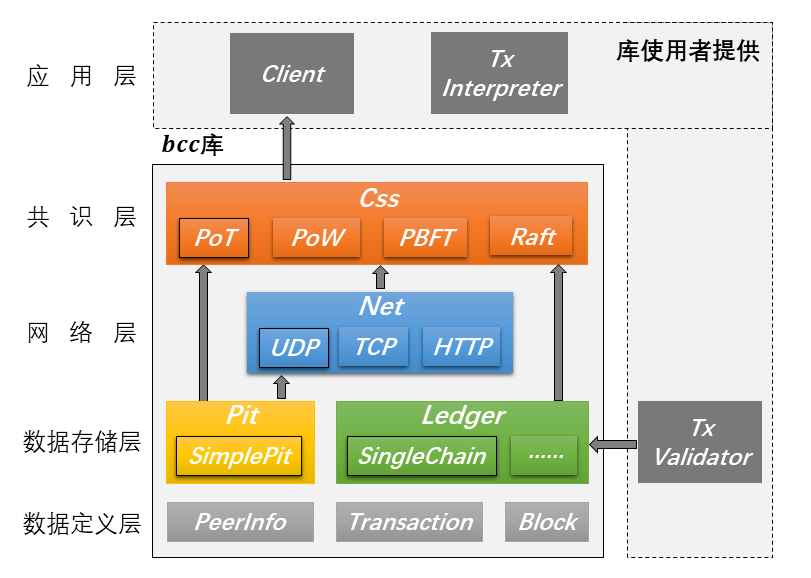
\includegraphics[width=0.7\columnwidth]{figure/chap5-bcc/fig-pot-bcc.png}}
	\caption{PoT协议模块结构}
	\label{fig:modules}
\end{figure}

\begin{enumerate}
    \item \textit{Css}。\textit{Css}模块即共识模块,是整个bcc库的核心。共识模块调用存储(\textit{Pit}、\textit{Ledger})与网络(\textit{Net})模块完成消息处理、状态转换、区块共识等任务。\textit{Css}的具体实现可以有PoT、PoW、PBFT、Raft等,目前默认提供了PoT实现。
	%\item \textit{Pot}. Pot模块是实现PoT协议的关键模块,其具体内容已在\ref{sec:pot-protocol}介绍。
	%Detailed below. The core module that implements the PoT protocol,
	      %which can essentially be seen as a state machine.
	\item \textit{Net}。\textit{Net}模块即网络模块,负责与其他节点的网络通信,包括消息格式的封装与解封、基础的验证工作等。\textit{Net}模块可以基于UDP、TCP、HTTP等多种协议实现。
	\item \textit{Pit}。\textit{Pit}即节点信息表(PeerInfoTable),负责存储集群所有节点必要的信息(如节点ID、节点网络地址等),并向\textit{Css}和\textit{Net}模块提供增删改查能力。\textit{Pit}的默认实现是\textit{SimplePit},对于需要记录节点信用历史、余额等的区块链项目可以自定义更丰富的\textit{Pit}模块。
	\item \textit{Ledger}。\textit{Ledger}即账本存储模块,负责区块与交易的增删改查操作,与\textit{Tx Validator}交互以验证新区块和新交易。\textit{Ledger}的默认实现是\textit{SimpleChain}(一个简单的区块链单链结构)。
	\item \textit{Client \& Tx Interpreter \& Tx Validator}。\textit{Client}(客户端模块)负责用户交互(构建交易、访问区块链信息等)。\textit{Tx Interpreter}(交易解释器)负责解释一个交易的内容。\textit{Tx Validator}(交易验证器)负责提供对交易的内容验证能力。这三项是基于bcc库构建区块链程序必须进行自定义的模块,并且交易验证器必须按照bcc库给出的接口定义进行实现,其他两个模块则是逻辑意义上的,由用户自行决定。%事实上,这三个模块在通过bcc库构建区块链程序时并不一定显示地
	%\item \textit{Tx Validator \& Interpreter}。这两个模块对于自定义应用而言非常重要,bcc库的使用者必须指定如何检验一个新交易是否合法、如何解释一个新交易的内容。
\end{enumerate}


\section{数据结构}

\subsection{账户ID}

\subsection{节点信息}

\subsection{交易}

\subsection{区块}

\subsection{消息}

\section{网络模块}

\subsection{BNet接口}

\subsection{TCPNet实现}

\subsection{UDPNet实现}

\section{节点表模块}

\subsection{Pit接口}

\subsection{SimplePit实现}

\section{账本模块}

\subsection{Ledger接口}

\subsection{SimpleChain实现}

\section{共识模块}

\subsection{Consensus接口}

\section{小结}

本章
